%%% Hlavní soubor. Zde se definují základní parametry a odkazuje se na ostatní části. %%%

%% Verze pro jednostranný tisk:
% Okraje: levý 40mm, pravý 25mm, horní a dolní 25mm
% (ale pozor, LaTeX si sám přidává 1in)
\documentclass[12pt,a4paper]{report}
\setlength\textwidth{145mm}
\setlength\textheight{247mm}
\setlength\oddsidemargin{15mm}
\setlength\evensidemargin{15mm}
\setlength\topmargin{0mm}
\setlength\headsep{0mm}
\setlength\headheight{0mm}
% \openright zařídí, aby následující text začínal na pravé straně knihy
\let\openright=\clearpage

\renewcommand\baselinestretch{1.3} % riadkovanie jeden a pol

%% Pokud tiskneme oboustranně:
% \documentclass[12pt,a4paper,twoside,openright]{report}
% \setlength\textwidth{145mm}
% \setlength\textheight{247mm}
% \setlength\oddsidemargin{15mm}
% \setlength\evensidemargin{0mm}
% \setlength\topmargin{0mm}
% \setlength\headsep{0mm}
% \setlength\headheight{0mm}
% \let\openright=\cleardoublepage

%% Pokud pouľíváte csLaTeX (doporučeno):
%\usepackage{czech}
%% Pokud nikoliv:
\usepackage[czech]{babel}
\usepackage[T1]{fontenc}

%% Pouľité kódování znaků: obvykle latin2, cp1250 nebo utf8:
\usepackage[utf8]{inputenc}

%% Ostatní balíčky
\usepackage{graphicx}
\usepackage{amsthm}
\usepackage{amssymb}
%\usepackage{alltt}
\usepackage{todonotes}
\usepackage{algorithmic}
\usepackage[chapter]{algorithm}

\renewcommand{\algorithmicrequire}{\textbf{Input:}}
\renewcommand{\algorithmicensure}{\textbf{Output:}}

\renewcommand{\algorithmicforall}{\textbf{for each}}

\renewcommand{\algorithmiccomment}[1]{// #1}

% pekne pokope definujeme potrebne udaje
\def\mftitle{Inference of an XML Schema with the Knowledge of XML Operations}
\def\mfthesistype{Master Thesis}
\def\mfauthor{Mário Mikula}
\def\mfadvisor{RNDr. Irena Mlýnková, Ph.D.}
\def\mfplacedate{Praha, 2011}

%% Balíček hyperref, kterým jdou vyrábět klikací odkazy v PDF,
%% ale hlavně ho pouľíváme k uloľení metadat do PDF (včetně obsahu).
%% POZOR, nezapomeňte vyplnit jméno práce a autora.
\usepackage[ps2pdf,unicode]{hyperref}   % Musí být za vąemi ostatními balíčky
\hypersetup{pdftitle=\mftitle}
\hypersetup{pdfauthor=\mfauthor}

%%% Drobné úpravy stylu

% Tato makra přesvědčují mírně oąklivým trikem LaTeX, aby hlavičky kapitol
% sázel příčetněji a nevynechával nad nimi spoustu místa. Směle ignorujte.
%\makeatletter
%\def\@makechapterhead#1{
%  {\parindent \z@ \raggedright \normalfont
%   \Huge\bfseries \thechapter. #1
%   \par\nobreak
%   \vskip 20\p@
%}}
%\def\@makeschapterhead#1{
%  {\parindent \z@ \raggedright \normalfont
%   \Huge\bfseries #1
%   \par\nobreak
%   \vskip 20\p@
%}}
%\makeatother

% Toto makro definuje kapitolu, která není očíslovaná, ale je uvedena v obsahu.
\def\chapwithtoc#1{
\chapter*{#1}
\addcontentsline{toc}{chapter}{#1}
}

\begin{document}

% Trochu volnějąí nastavení dělení slov, neľ je default.
\lefthyphenmin=2
\righthyphenmin=2

%%% Titulní strana práce

\pagestyle{empty}
\begin{center}

\large

Charles University in Prague

\medskip

Faculty of Mathematics and Physics

\vfill

{\bf\Large \mfthesistype}

\vfill

\centerline{\mbox{
\includegraphics[width=60mm]{logo.eps}}}

\vfill
\vspace{5mm}

{\LARGE \mfauthor}

\vspace{15mm}

% Název práce přesně podle zadání
{\LARGE\bfseries \mftitle}

\vfill

% Název katedry nebo ústavu, kde byla práce oficiálně zadána
% (dle Organizační struktury MFF UK)
Katedra softwarového inženýrství

\vfill

\begin{tabular}{rl}

Supervisor of the master thesis: & \mfadvisor \\
\noalign{\vspace{2mm}}
Study programme: & Informatika \\
\noalign{\vspace{2mm}}
Specialization: & ISS \\
\end{tabular}

\vfill

% Zde doplňte rok
\mfplacedate

\end{center}

\newpage

%%% Následuje vevázaný list -- kopie podepsaného "Zadání diplomové práce".
%%% Toto zadání NENÍ součástí elektronické verze práce, nescanovat.

%%% Na tomto místě mohou být napsána případná poděkování (vedoucímu práce,
%%% konzultantovi, tomu, kdo zapůjčil software, literaturu apod.)

\openright

\noindent
\todo[inline]{Poďakovanie.}

\newpage

%%% Strana s čestným prohláąením k diplomové práci

\vglue 0pt plus 1fill

\noindent
I declare that I carried out this master thesis independently, and only with the cited
sources, literature and other professional sources.

\medskip\noindent
I understand that my work relates to the rights and obligations under the Act No.
121/2000 Coll., the Copyright Act, as amended, in particular the fact that the Charles
University in Prague has the right to conclude a license agreement on the use of this
work as a school work pursuant to Section 60 paragraph 1 of the Copyright Act.

\vspace{10mm}

\hbox{\hbox to 0.5\hsize{%
In ........ date ............
\hss}\hbox to 0.5\hsize{%
Signature
\hss}}

\vspace{20mm}
\newpage

%%% Povinná informační strana diplomové práce

\vbox to 0.5\vsize{
\setlength\parindent{0mm}
\setlength\parskip{5mm}

Název práce:
\mftitle
% přesně dle zadání

Autor:
\mfauthor

Katedra:  % Případně Ústav:
Název katedry či ústavu, kde byla práce oficiálně zadána
% dle Organizační struktury MFF UK

Vedoucí diplomové práce:
\mfadvisor, pracoviště
% dle Organizační struktury MFF UK, případně plný název pracoviątě mimo MFF UK

Abstrakt:
% abstrakt v rozsahu 80-200 slov; nejedná se vąak o opis zadání diplomové práce

Klíčová slova:
% 3 aľ 5 klíčových slov

\vss}\nobreak\vbox to 0.49\vsize{
\setlength\parindent{0mm}
\setlength\parskip{5mm}

Title:
% přesný překlad názvu práce v angličtině

Author:
\mfauthor

Department:
Název katedry či ústavu, kde byla práce oficiálně zadána
% dle Organizační struktury MFF UK v angličtině

Supervisor:
\mfadvisor, pracoviště
% dle Organizační struktury MFF UK, případně plný název pracoviątě
% mimo MFF UK v angličtině

Abstract:
% abstrakt v rozsahu 80-200 slov v angličtině; nejedná se vąak o překlad
% zadání diplomové práce

Keywords:
% 3 aľ 5 klíčových slov v angličtině

\vss}

\newpage

%%% Strana s automaticky generovaným obsahem diplomové práce. U matematických
%%% prací je přípustné, aby seznam tabulek a zkratek, existují-li, byl umístěn
%%% na začátku práce, místo na jejím konci.

\openright
\pagestyle{plain}
\renewcommand\thepage{}
\tableofcontents
\newpage
\renewcommand\thepage{\arabic{page}}
\setcounter{page}{1}

\newtheorem{theorem}{Theorem}
\theoremstyle{definition}
\newtheorem*{define}{Definition}	% Definice nečíslujeme, proto "*"
\newtheorem{example}{Example}


%%% Jednotlivé kapitoly práce jsou pro přehlednost uloľeny v samostatných souborech
%\include{uvod}
\chapter{Analysis of Recent Approaches} \label{chapter_analysis_of_recent_approaches}
Approaches of XML schema inference can be divided by several criteria. A basic division is by the language the resulting schema is written in. Commonly used languages are DTD and XML Schema.

According to \cite{Mlynkova:2008:AAX:1494650.1495496}, the type of the inference method can be divided into \emph{heuristic} and \emph{grammar-inferring}. Heuristic methods are based on experience with manual construction of schemas, motivated by real-world usages of XML schema, and their result commonly does not belong to any class of grammar. On the contrary, the grammar-inferring methods are based on theoretical knowledge of automata and their results belong to a particular class of languages. Thus, these methods guarantee specific characteristics of the results. \todo[inline]{Tady by neškodilo dát odkazy na všechny ex. přístupy a říct, že popíšeme detailněji aspoň dva.}

Another important criterion is the type of input data. Most of the approaches process XML documents as the input of the inference process and the documents are supposed to be valid against the resulting schema. Besides approaches exploiting XML data, approaches that utilize other or additional sources may be developed. An approach utilizing XML data along with an obsolete XML schema is described in \cite{Mlynkova:2009:IXS:1862681.1862693}. However, the most significant approaches in terms of this work are those, utilizing operations over XML data. According to our best knowledge at the time of writing, there is just one approach of this category, described in \cite{Necasky:2009:DXK:1529282.1529414}. It utilizes a set of XQuery queries to discover keys and foreign keys\todo{ref do literatury - Ty by tady něškodily všude, u každé té kategorie.}.

\section{Common Caracteristics}
The process of inference commonly used by a significant number of approaches is summarized in \cite{Mlynkova:2008:AAX:1494650.1495496} as the following one: For each occurrence of element $e$ from the input XML documents and its subelements $e_1, e_2, ..., e_k$ a production $e \rightarrow e_1 e_2 ... e_k$ is constructed. The productions form so-called \emph{initial grammar} (IG). For each element type the productions are then merged, simplified and generalized using various methods and criteria. A common approach is so-called \emph{merging state algorithm}, where a \emph{prefix tree automaton} (PTA) is built from the productions of the same element type and the automaton is generalized via merging of its states. Finally, the generalized automaton/grammar is expressed in syntax of the respective XML schema language.
\todo[inline]{Tento odstavec je doslovne prebraty z uvedeneho clanku. Mozem to takto pouzit?}

\section{XTRACT}
The XTRACT \cite{Garofalakis:2000:XSE:342009.335409} system is an example of a \emph{heuristic} \emph{merging state algorithm} creating the result in DTD. Its process of inference consists of three steps:
\begin{enumerate}
\item Generalization - Generates a set of DTD candidates by searching the input for certain patterns and generalising corresponding fragments using regular expressions.
\item Factoring - Groups of generalized candidate DTDs are factorized to a new ones by finding common sub-expressions to make them more concise.
\item Minimum Description Length (MDL) Principle - Composing a near-optimal DTD schema from the set of all generalized candidate DTDs.
\end{enumerate}

\subsection{Generalization}
Purpose of generalization is to create a set of DTD candidates - schemata that cover fractions of the input XML data. In the last step, this set will be used to compose a (sub)optimal result with respect to a trade-off between its preciseness and conciseness. Therefore, it is desirable to create DTD canditates with various degree of these two characteristics.

Generalization is based on replacing fragmets (sequences of subelements of a given element) from the input XML data by regular expressions, thus, using metacharacters like (*, +, ?). To provide a wide set of DTD canditates, each sequence is processed several times using various values of input parameters. Due to the very large number of possible DTD canditates, the authors employ certain real-life motivated heuristics.

For instance, the paper (\cite{Garofalakis:2000:XSE:342009.335409}) introduces the following example: Sequences \texttt{abab} and \texttt{bbbe} are generalized to \texttt{(ab)*}, \texttt{(a|b)*}, \texttt{b*e}.
\todo[inline]{Mozem takto pouzivat prevzate priklady?}

\subsection{Factoring}
Factoring is a process of creating a new DTD canditate from two or more DTD canditates, decresing their summed size without modifications in their semantics. An aim of this step is to decrease a MDL cost of DTD candidates calculated in the MDL step and thus refine the process of construction of the resulting DTD.

An example introduced it the paper (\cite{Garofalakis:2000:XSE:342009.335409}): DTD candidates \texttt{ac}, \texttt{ad}, \texttt{bc} and \texttt{bd} are factored into \texttt{(a|b)(c|d)}.

Alike the generalization step, also in this step the set of possible factored DTD is huge and the authors propose certain heuristics to make the factorization effective.

\subsection{Minimum Description Length (MDL) Principle}
This is an important step trying to create the resulting DTD with the best trade-off between its preciseness and conciseness.  

Paper \cite{Mlynkova:2008:AAX:1494650.1495496} summarizes this step as follows: It expresses the quality of a DTD candidate using two aspects – conciseness and preciseness. Conciseness of a DTD is expressed using the number of bits required to describe the DTD (the smaller, the better). Preciseness of a DTD is expressed using the number of bits required for description of the input data using the DTD. In other words, the more accurately the structure is described, the fewer bits are required. Since the two conditions are contradictory, their balancing brings reasonable and realistic results.

\todo[inline]{Detailnejsie? Priklad?}

\section{Even an Ant Can Create an XSD}
This work, described in \cite{Vosta:2008:EAC:1802514.1802522}, combines several previously proposed approaches including the XTRACT system discussed in the previous section. Its improvements of the process of XML schema inference include:

\begin{itemize}
\item Distinguishing elements with the same name but different semantics.
\item Improvements of algorithms adopted from the previous works.
\item Incorporating inference of an unordered sequence.
\item Creating a result in XML Schema language.
\end{itemize}

\subsection{Clustering of Elements}
This phase clusters elements on a basis of their context and structure. It is done by creating tree structures for each input XML documents, where vertices represent elements and attributes and an edge between two vertices expresses the their parent-child relation. These trees and their subtrees and then compared, using an imposed tree similarity measure, to find elements with the same semantics.

\subsection{Schema Generalization}
For each cluster, a trivial schema is created, which is then generalized to achieve a reasonable result. In a search for the optimal schema, \emph{Ant Colony Optimization (ACO)} heuristic is incorporated. The idea behind the ACO heuristic is that a set of artifical ants is searching a space of possible solutions, each ant given a subspace of the space to find a local suboptimum. An ant 
is performing steps (schema modifications), dying after a predifined number of steps and providing an information - positive feedback - on quality of a found solution. The search is performed in a defined count of interations (or it stops if good enough solution is found) and the positive feedback from one iteration is used to find better results in the following iterations. Every step of an ant represents a modification of a schema, in particular, a merge of states in a corresponding PTA.

One of the improvements of this heuristic is inclusions of a negative feedback after each step of an ant, visible only in a current iteration. Due to this improvement, a larger subspace of solutions is searched.

Another improvement lies in a way how an ant decides for a particular step to perform. To achieve better results, the authors propose a combinations of several verified approaches. A set of all possible steps is created using \emph{k,h-context} and \emph{s,k-string} \todo{citacie} methods. The optimal step is then selected employing the MDL principle \todo{citacia}.

\subsection{Result in XSD}
Unlike the majority of recent approaches, this methods creates its result in XML Schema language (XSD). Comparing to DTD, XSD is a newer language and it provides greater expression possibilities. Authors of this method focused on inferring elements with the same name but different context and the unordered sequences which can be in XSD expressed by \texttt{xs:all} construct. Elements with the same name but different context cannot be expressed in DTD and, however, the unordered sequence can be also expressed in DTD as alternations of ordered sequences, such expression in not practical nor well human-readable.

\section{On Inference of XML Schema with the Knowledge of an Obsolete One}
\todo[inline]{spravne zaradit}
An aim of approach described in \cite{Mlynkova:2009:IXS:1862681.1862693} is to exploit an obsolete XML schema as an additional input information to infer a new schema more efficiently. A XML schema can become obsolete due to changes in a set of XML documents, without capturing these changes in the schema. Thus, the schema becames outdated and according to the paper, this case is quite common.

On input, the method is given:
\begin{itemize}
\item An original XML schema.
\item A set of XML documents. Not all have to be valid against the original schema.
\end{itemize}

And the algorithm consists of two independent steps:

\begin{enumerate}
\item Correction of the input schema.
\item Specialization of the input schema.
\end{enumerate}

In the fist step the input schema is corrected to conform to the whole set of input XML documents. This is done by creating a PTA \todo{ref na def} for each production extracted from the input schema and merging it with a respective production from the initial grammar \todo{ref na def}, involving ACO and MDL heuristics.

In the second step, assuming a correct schema it is wanted to specialize the REs involved in the schema with regard to the XML documents, resulting in more precise and readable schema. Optional substeps are pruning of unused schema fragments, correction of lower and upper bounds of occurrences, transcription of operators to a more restrictive but simplier form, if this transcription preserves the validity, and refactorization to improve readability.

\section{Discovering XML Keys and Foreign Keys in Queries}
This method is described in paper \cite{Necasky:2009:DXK:1529282.1529414}. It tries to improve automatic XML schema inference by discovering keys and foreign keys from a set of XQuery queries. Just the queries are utilized in inference, no XML data are used. The output of this method is a set of keys and foreign keys that can be captured using XML Schema \textbf{key}, \textbf{keyref} and \textbf{unique} constructs.

\subsection{Assumptions and Observations}
To discover keys and foreign keys, the method utilizes element/element joins. Assume a query $Q$ that joins a sequence of elements $S_1$ targeted by a path $P_1$ with a sequence of elements $S_2$ targeted by a path $P_2$ on a condition $L_1 = L_2$.
\todo[inline]{priklad}
The method is based on assumption that each join is done via key/foreign key pair. It means it is supposed that $L_1$ is a key of the elements $S_1$ and $L_2$ is it's respective foreign key or vice versa.

The author describe two possible cases:

\begin{enumerate}
\renewcommand{\theenumi}{(O\arabic{enumi})}
\renewcommand{\labelenumi}{\theenumi}
\item $L_1$ is a key of the elements $S_1$, $L_2$ is a respective foreign key and it itself is not a key of the elements $S_2$.
\item $L_2$ is a key of the elements $S_2$, $L_1$ is a respective foreign key and it cannot be decided whether $L_1$ is a key of the elements $S_1$ or not.
\end{enumerate}

\subsection{Join Patterns and Key Inference}
For a certain join, the decision for one of the cases (O1) and (O2) is made by the form of the join. The query is searched for so-called \emph{join patters}. These are \emph{for join pattern} and \emph{let join pattern} and they are as follows (the first is \emph{for join pattern}, \emph{let join pattern}):

\todo[inline]{spravne kreslit indexy pri pismenkach}
\begin{verbatim}
for $e1 in P1              for $e1 in P1
return                     return
    for $e2 in                 let $e2 :=
        P2[L2 = $e1/L1]            P2[L2 = $e1/L1]
    return CR                  return CR
\end{verbatim}

Each occurrence of a join pattern is classified by application of the following rules it this specific order. The first satisfied ruled is applied. The occurrence is also assigned with a weight determining how sure the method is about the inferred statement.

The pattern occurrence is considered of case (O1) if it is the for join pattern (weight: 1), if aggregation function \texttt{avg}, \texttt{min}, \texttt{max} or \texttt{sum} is applied on a return path (weight: 1) or if aggregation function \texttt{count} is applied on a return path (weight: 0.75). \todo {definovat return path?}

Else, the pattern occurrence is considered of case (O2) and the assigned weight depends on the number of target return paths. If the number is greater than one, the weight is one (weight: 1), else (the number is less or equal one) the weight is one half (weight: 0.5).

\subsection{Summarization of the Results}

The assumption the method is based on may not be fulfilled for every join in a supplied set of queries. A key $K$ may be inferred from some query and processing of another query may result to denial of $K$ as a key. \todo[inline]{priklad?}

Therefore, the authors introduce a scoring function to summarize the positive and the negative statements about keys using the assigned weights. The value of the score expresses the probalitity that a respective key statement is satisfied. Finally, the scores of the inferred keys are normalized to be comparable with each other.

\subsection{Conclusion}
The output of the method is a list of scored keys and for each key a list foreign keys referencing the key. Since the method deals only with the inference of keys, it is not an overall method of the XML schema inference. It is meant to be used in a collaboration with other schema-inferring methods to refine their results.

Since the method is based on intuition of how XQuery constructs are commonly applied in practice, it can be imprecise in certain cases.

\todo[inline]{Tady by se hodila nějaká srovnávací tabulka metod z různách pohledů (metoda, vstupy, výstupy). Dále pak kapitola na téma co dnešní metody neumí a čím se tedy v práci budeme zbývat. Tj. Nějaká návaznost k další kapitole.}
%\chapter{Basic Definitions}

In this chapter basic definitions necessary in the following chapters are placed. The definitions are taken from \cite{RepAndConsistentAnswer, QueryXML, ImprovingXML}.


\section{XML Trees and DTDs}
\begin{define}[Tree]
Being given an alphabet of nodes $\mathbb{N}$ and an alphabet of node labels $\Sigma$, a {\sl tree} $T$ over $\mathbb{N}$ and $\Sigma$ is a tuple $(r_T, N_T, E_T, \lambda_T)$, where $N_T \subseteq \mathbb{N}$ is the set of nodes, $\lambda_T : N_T \to \Sigma$ is a node labelling function, $r_T \in N_T$ is the distinguished root of $T$, and $E_T \subseteq N_T \times N_T$ is a set of edges such that starting from any node $n_i \in N_T$ it is possible to reach any other node $n_j \in N_T$, walking through a sequence of edges $e_1,\dots,e_k$ which are connected and acyclic.\qed
\end{define}

\noindent Let us also denote the set of leaf nodes as $Leaves(T)$ and the set of trees defined over an alphabet of node labels $\Sigma$ as $T_\Sigma$.

\begin{define}[XML Tree]\label{xmlTree}
{\sl XML tree} is a pair $XT=\langle T,\delta \rangle$, where:
\renewcommand{\labelenumi}{\roman{enumi})}
	\begin{enumerate}
		\item $T = (r, N, E, \lambda)$ is a tree from $T_{\tau\cup\alpha\cup\{S\}}$, where $\tau$ is a tag alphabet, $\alpha$ is an attribute name alphabet and $S$ is a symbol not belonging to $\tau\cup\alpha$ (representing \texttt{\#PCDATA} content of elements)$;$
		\item given a node $n$ of $T$, $\lambda(n) \in \alpha \cup \{S\} \Leftrightarrow n \in Leaves(T);$
		\item $\delta : Leaves(T) \rightarrow Str$ where $Str$ is a string alphabet is a function associating a (string) value to every leaf of $T$.
	\end{enumerate}\qed
\end{define}

\begin{example}\label{example1ref}
Consider the following XML document representing a collection of books. Its graphical representation as an XML tree is in Fig. \ref{example1}.
\begin{verbatim}
<bib>
  <book>
    <written_by>
      <author ano="A1">
        <name>John Writer</name>
      </author>
      <author ano="A1">
        <name>Eric Seller</name>
      </author>
    </written_by>
    <title>Some title</title>
  </book>
  <book>
    <written_by>
      <author ano="A2">
        <name>Adam Publisher</name>
      </author>
    </written_by>
    <title>Some title 2</title>
  </book>
</bib>
\end{verbatim}

The nodes of an XML tree have a label denoting the tag name of the element and unique element identifier in brackets. Leaf nodes are either an attribute or the textual content of an element. The label of a textual node contains string contained inside of element and unique element identifier. The label of an attribute node contains in addition to textual node the name of the attribute.\qed
\end{example}

\begin{figure}[h]
    \centering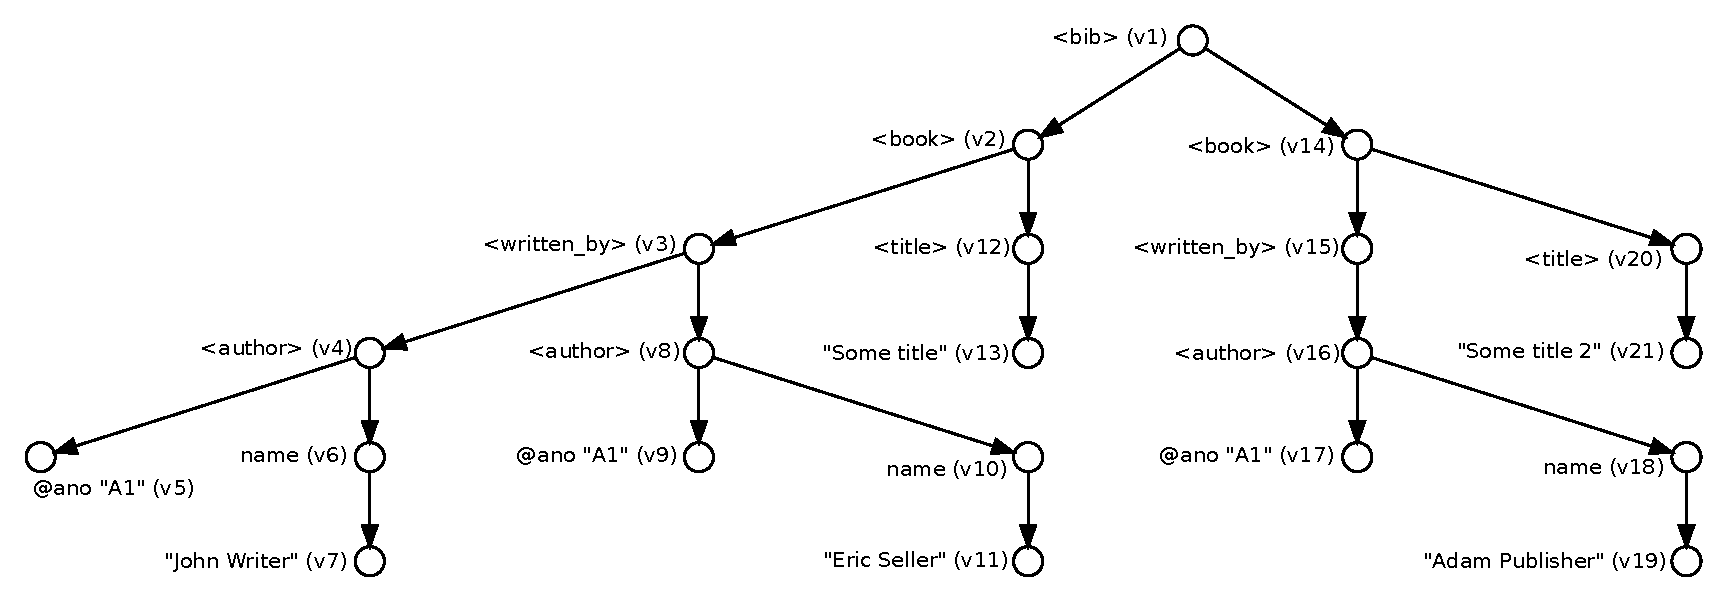
\includegraphics[width=\textwidth]{example1-new}
	\caption{An XML Tree} \label{example1}
\end{figure}

\begin{define}[DTD]\label{dtdDef}
{\sl DTD} is a tuple $D = (\tau, \alpha, P, R, rt)$ where:
\renewcommand{\labelenumi}{\roman{enumi})}
\begin{enumerate}
	\item $\tau$ and $\alpha$ are of the same definition as in the \emph{XML tree}
    \item $P$ is the set of \emph{element type definitions}
    \item $R$ is the set of \emph{attribute lists}
    \item $rt \in \tau$ is the tag of the document root element.
\end{enumerate}
\qed
\end{define}

\begin{define}[Path Expression]
A {\sl path expression} is an expression of the form $p = ('/' | '//')s_1 \dots ('/'|'//')s_m$ where $s_1, \dots, s_{m-1} \in \tau$, and $s_m \in \tau \cup \alpha \cup \{S\}$.\qed
\end{define}

\begin{define}[Path]
{\sl Path} p on a DTD $D = (\tau, \alpha, P, R, rt)$ is a sequence $p = s_1, \dots, s_m$ of symbols in $\tau \cup \alpha \cup \{S\}$ such that:
\renewcommand{\labelenumi}{\roman{enumi})}
	\begin{enumerate}
		\item $s_1=rt$;
		\item for each $i$ in $2..m-1$, $s_i \in \tau$ and $s_i$ appears in the element type definition of $s_{i-1}$;
		\item $s_m \in \alpha \Rightarrow s_m$ appears in the attribute list of $s_{m-1}$;
		\item $s_m \in \tau \cup \{S\} \Rightarrow s_m$ appears in the element type definition of $s_{m-1}$.
	\end{enumerate}\qed
\end{define}

As we have defined a \emph{path} on a DTD $D$, let us denote $paths(D)$ as the set of all paths which can be defined on a DTD $D$. Also, another important notion is $p(XT)$ (or $\{[\![p]\!]\}$), which is the set of nodes from XML tree $XT$ conforming to DTD $D$, which can be reached by the path $p \in paths(D)$, starting from the root of $XT$. The set of nodes reachable from a node $v$ following path $p$ is denoted as $\{v[\![p]\!]\}$. When there is only one node in $\{v[\![p]\!]\}$, we use $v[\![p]\!]$ to denote this node. Moreover, let $XT.p$ denote the \emph{answer} of the path $p$ applied on $XT$ that is:
\begin{itemize}
	\item if $p \in EPath(D)$, where $EPath(D)$ denotes the set of the paths whose last symbol denotes an element, then $XT.p = p(XT)$
	\item if $p \in StrPath(D)$, where $StrPath(D)$ denotes the set of paths whose last symbol denotes either the textual content of an element or an
attribute, then $XT.p = \{\delta_T(x)|x \in p(XT)\}$.
\end{itemize}

\begin{example}\label{pathExample}
Consider the XML tree $XT$ from Example \ref{example1ref} conforming the DTD $D$ defined below, which is representing a collection of books.
\begin{verbatim}
<!ELEMENT bib (book+)>
<!ELEMENT book (written_by, title)>
<!ELEMENT written_by (author+)>
<!ELEMENT author (name)>
<!ATTLIST author ano CDATA>
<!ELEMENT name PCDATA>
<!ELEMENT title PCDATA>
\end{verbatim}

The set $paths(D)$ contains the following paths:
\begin{align}
paths(D) &= \left\{/bib, /bib/book, /bib/book/written\_by,\right.\nonumber\\
&\qquad \left. /bib/book/written\_by/author, \right.\nonumber\\
&\qquad \left. /bib/book/written\_by/author/name, \right.\nonumber\\
&\qquad \left. /bib/book/written\_by/author/name/S, \right.\nonumber\\
&\qquad \left. /bib/book/written\_by/author/@ano, \right.\nonumber\\
&\qquad \left. /bib/book/title, /bib/book/title/S\nonumber\right\}
\end{align}\qed
\end{example}

\section{Integrity Constraints}

Before defining of the XML integrity constraint, let us introduce some notation used in the definition. A \emph{path atom} is an expression of the form $[x_1]p[x_2]$, where $p$ is a path expression, $x_1$ and $x_2$ are terms, and $x_1 \not \in Str$.\\
A conjunction of path and built-in atoms $C = [X_1]p_1[Y_1] \cap \dots \cap [X_n]p_n[Y_n] \cap U_1\theta_1 V_1 \cap \dots \cap U_k \theta_k V_k$ is said to be \emph{safe} if all variables in $C$ are \emph{range restricted}, i.e. if
\begin{itemize}
 	\item for every $[X_i]p_i[Y_i]$, either $X_i$ is a constant (node identifier of a string), or there is some $[X_j]p_j[Y_j]$ in $C$ where $X_j$ is range restricted;
    \item for every built-in term $U_i\theta_i V_i$ occurring in $C$, if $\theta_i$ is equal to $"="$ then at least one of the two terms is range restricted; otherwise both $U_i$ and $V_i$ must be range restricted.
 \end{itemize}

A rootless tree formula is an expression of the form $p(\Phi_1 \land \dots \land \Phi_k)$ where $\Phi_i$ is a rootless path formula (expression of the form $p[y]$ where $p$ is a path expression and $y$ is a term) or a rootless tree formula and $p$ is a path expression. A tree atom is an expression of the form $[x]T$ where $T$ is a rootless tree formula and $x$ is a term.

\begin{define}[XML Integrity Constraint]\label{integConstr}
An {\sl XML constraint} is a formula of the form: $$(\forall X)[\Phi(X)\supset (\exists Y_1)\Psi_1(X,Y_1) \lor \dots \lor (\exists Y_k)(X,Y_k)]$$
where $X,Y_1,\dots, Y_k$ denote distinct sets of universally and existentially quantified variables, $\Phi(X)$ and $\Phi(X) \land \Psi_i(X, Y_i) (\forall i \in [1..k])$ are safe conjunctions of built-in and tree atoms.\qed
\end{define}

\begin{example}
Consider the XML tree $XT$ from Example \ref{example1ref}. Thereafter the integrity constraint that there must exist at least two books differents titles is expressed as

\begin{align*}
\forall(X)&[[root]/bib[X] \supset\\
&\exists(Z_1, Z_2)([X]/book/title/S[Z_1] \land [X]/book/title/S[Z_2] \land Z_1 \not = Z_2)]
\end{align*}
\end{example}

\section{Functional Dependencies}

Since different approaches uses slightly different representation of an XML document, also the definition of functional dependencies differs, too. This is the reason why we introduce two different definitions in this section.

\subsection{Functional Dependency 1}

In a relational database, a correspondence between values $A$ and $B$ in the tuple of $D$ models the functional dependency denoted as $A \rightarrow B$. Since in XML there is no such standard tuple concept, the concept of XML tree tuples is introduced, corresponding to the concept of tuples in relational databases.

\begin{define}[Tree Tuple]\label{treeTuple}
Being given an XML tree $XT$ conforming to DTD $D$, a {\sl tree tuple} $t$ of $XT$ is a maximal sub-tree of $XT$ such that for every path $p \in paths(D)$, $t.p$ contains at most one element.\qed
\end{define}

\begin{example}
Consider the XML tree $XT$ in Fig. \ref{example1}. The subtrees of $XT$ shown in Fig. \ref{tuples} are tree tuples, and the subrees in Fig. \ref{nottuples} are not.

\begin{figure}[H]
    \centering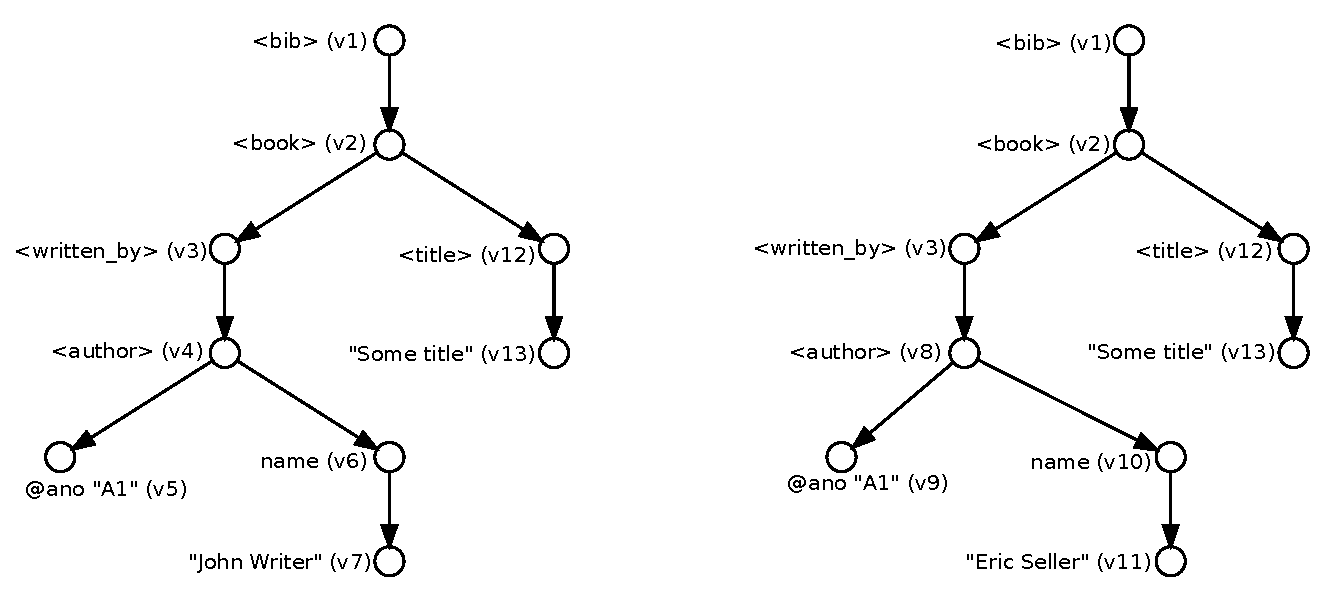
\includegraphics[width=\textwidth]{tuples}
	\caption[Two tree tuples of the XML tree]{Two tree tuples of the XML tree in Fig. \ref{example1}} \label{tuples}
\end{figure}

\begin{figure}[H]
    \centering
    \subfloat[]{\label{nottuple1}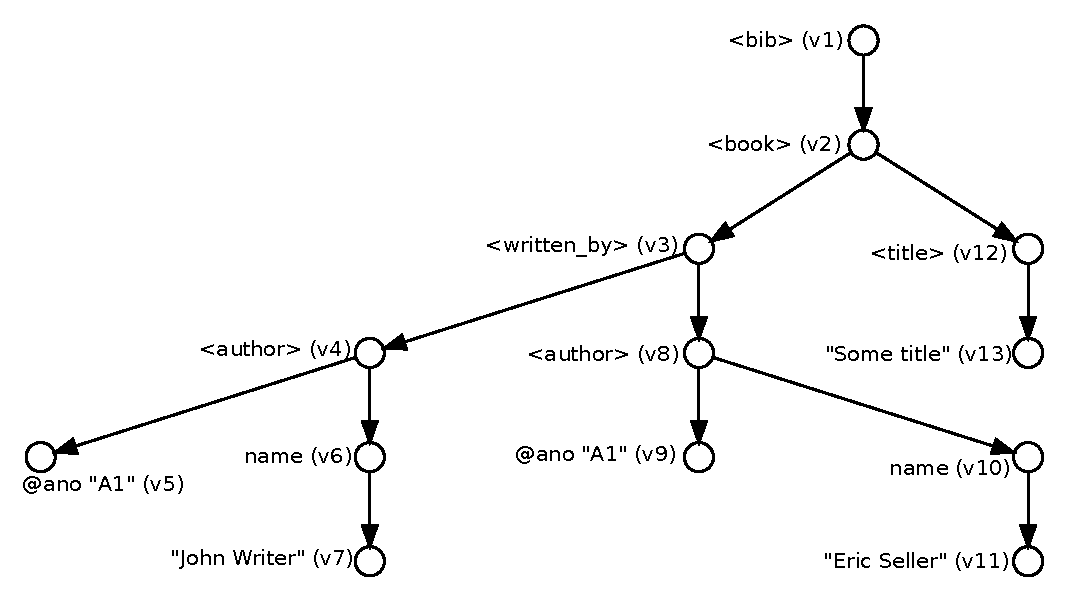
\includegraphics[scale=0.6]{nottuples1}}
    \subfloat[]{\label{nottuple2}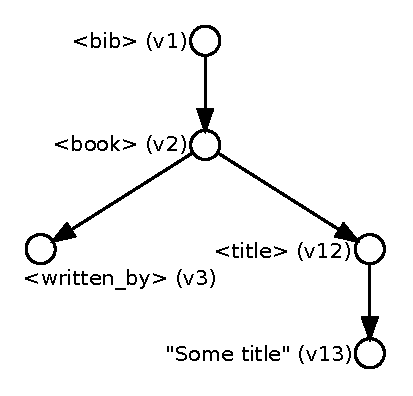
\includegraphics[scale=0.6]{nottuples2}}
	\caption[Two subtrees of the XML tree]{Two subtrees of the XML tree in Fig. \ref{example1} which are not tree tuples}
    \label{nottuples}
\end{figure}

In Fig. \ref{nottuple1}, the subtree is not a tree tuple, because the answer of the path $/bib/book/written\_by/author$ contains two distinct nodes (i.e. $v4$ and $v8$). The subtree in the Fig. \ref{nottuple2} is not a tree tuple, because it is not a maximal subtree (it is a subtree of a tuple from Fig. \ref{tuples}).\qed

\end{example}

\begin{define}[Functional Dependency]\label{fd1}
Being given a DTD $D$, a {\sl functional dependency} on $D$ is an expression of the form $S \rightarrow p$, where $S$ is a finite non empty subset of $paths(D)$ and $p \in paths(D)$.\qed
\end{define}

\begin{example}\label{fdExample}
Consider the XML tree in Fig \ref{example1}. The following functional dependency expresses the constraint that two distinct authors of the same book cannot have the same value of attribute \texttt{ano}:$$\{/bib/book, /bib/book/written\_by/author/@ano\} \rightarrow /bib/book/written\_by/author$$\qed
\end{example}

\subsection{Functional Dependency 2}

\begin{define}[Functional Dependency]\label{fd2}
With a given DTD $D$, a {\sl functional dependency} is of the form $\sigma = (P, P', (P_1, \dots, P_n \rightarrow P_{n+1}))$. Here $P$ is a  root path (path where the first element is a root element of an XML document), or $P = \epsilon$ (empty path). Each $P_i (i \in [1,n])$ is a singleton leaf path, and there is a no non-empty common prefix for $P_1, \dots, P_{n+1}$. Being given an XML document $T$ conforming to $D$, we say $T$ satisfies $\sigma$:iff $\forall v \in \{[\![P]\!]\}, \forall v_1, v_2 \in \{v[\![P']\!]\}$, if $v_1[\![P_i]\!] \equiv v_2[\![P_i]\!]$ for all $i \in [1,n]$, then $v_1[\![P_{n+1}]\!] \equiv v_2[\![p_{n+1}]\!]$.\qed
\end{define}

The main difference between two definitions of the functional dependency is that the former definition can use any path from $paths(D)$, whereas the latter considers that each $P_i (i \in [1,n])$ is from $StrPaths(D)$. That means the constraint from Example \ref{fdExample} cannot be expressed by functional dependency defined in \ref{fd2}, because of $/bib/book/written\_by/author$ path. Nevertheless, modified constraint from Example \ref{fdExample} expressed by FD defined in \ref{fd2} is shown in Example \ref{fd2Example}.

\begin{example}\label{fd2Example}
Consider the constraint $C$ saying that two distinct authors with different names of the same book cannot have the same value of attribute \texttt{ano}. The functional dependency expressing $C$ is defined as follows:

$$(bib/book, written\_by/author, (@ano \rightarrow name))$$\qed
\end{example}

%\chapter{Analysis of Recent Approaches}

This chapter introduces description and categorization of recent approaches of repairing XML documents with usage of functional dependencies.

All approaches dealing with the problem of finding optimal repair can be divided into categories according to usage of elementary repair primitives. This repair primitives are: inserting node, deleting node, updating node and marking node as unreliable of XML document.

\section[Repairs and Consistent Answers for XML Data]{Repairs and Consistent Answers for XML Data with Functional Dependencies}

A technique for computing repairs which solves the problem of XML data inconsistency with respect to a set of functional dependencies was proposed in \cite{RepAndConsistentAnswer}. In this approach, the authors are trying to find a minimal set of update operations which makes XML data consistent. These update operations can be divided into two categories i) replacing a value associated with an element or an attribute, and ii) marking a particular node information as unreliable.

\subsection{XML Tree and Functional Dependency}

To be able to resolve problem of functional dependency violations in XML document, the authors try to introduce the concept of functional dependendenies based on those defined for relational databases. Concept of a tree tuple and functional dependency is defined in Definition \ref{treeTuple} and \ref{fd1}.

Given an XML tree $XT$ conforming a DTD $D$ and a functional dependency $F : S_1 \rightarrow S_2$ , we say that $XT$ satisfies $F (XT \models F )$ if for each pair of tree tuples $t_1, t_2$ of $XT$, $t_1.S_1 = t_2.S_1 \land t_1.S_1 = \emptyset \Rightarrow t_1.S_2 = t_2.S_2$ . Given a set of functional dependencies $\mathcal{FD} = \{F_1 , \dots, F_n\}$ over $D$, we say that $XT$ satisfies $\cal FD$ if it satisfies $F_i$ for every $i \in 1..n$.

\subsection{Repairing inconsistent XML data}

Authors of this approach chose two kinds of actions to repair inconsistent XML data with regard to functional dependencies. The first action is updating the value of an attribute or content of an element. As the second action authors choose marking inconsistent element as "unreliable" rather than deleting it, because removing elements from an XML document leads to some undesired drawbacks: it does not always suffice to remove inconsistency and deleting a node can lead to a new document not valid against the given schema.

Depending on XML data and defined functional dependencies, each inconsistency could have many possible strategies to repair it. From all the possible repair strategies, the authors prefer those, for which smaller changes are made to the original document.

\begin{example}
Consider XML tree $XT$ from Example \ref{example1ref} conforming the DTD $D$ defined below, which is representing collection of books and the following functional dependency:\\ $\{bib.book, bib.book.written\_by.author.@ano\} \rightarrow bib.book.written\_by.author$.
\begin{verbatim}
<!ELEMENT bib (book+)>
<!ELEMENT book (written_by, title)>
<!ELEMENT written_by (author+)>
<!ELEMENT author (name)>
<!ATTLIST author ano CDATA>
<!ELEMENT name PCDATA>
<!ELEMENT title PCDATA>
\end{verbatim}
The functional dependency defined above requires that for each book, there is only one element author having a given $@ano$ value. Therefore $XT$ does not satisfy the given functional dependency, because two author elements of the same book have the same value of attribute $@ano$. To resolve this data inconsistency, we can use two different repair strategies: 1) changing one of the value of attribute $@ano$; 2) marking one of the element author as unreliable. Since the first strategy changes only attribute $@ano$, it is preferred to second strategy, which changes a larger portion of document, since it marks whole author element as unreliable.
\qed
\end{example}


\subsection{Repair Algorithm}

Before introducing the algorithm to repair inconsistent XML document, let us define reliability of elements in XML tree:

\begin{define}[R-XML Tree]
A R-XML $tree$ is a triplet $RXT = \langle T, \delta, \varrho \rangle$, where $\langle T, \delta \rangle$ is an XML tree and $\varrho$ is a reliability function from $N_T$ to \texttt{\{true, false\}}, such that, for each pair of nodes $n_1 , n_2 \in N_T$ with $n_2$ descendant of $n_1$, it holds that $\varrho(n_1) = false \Rightarrow \varrho(n_2) = false$.\qed
\end{define}

To be able to create a repair, R-XML Tree must not satisfy FD according to definition of weak satisfiability:

\begin{define}[Weak satisfiability]
Let $RXT = \langle T, \delta, \varrho \rangle$ be an R-XML tree conforming a DTD $D$, and $f: S \rightarrow p$ be a functional dependency. We say that $RXT$ weakly satisfies $f$ ($RXT \models_w f$) if one of the following conditions holds:
\begin{enumerate}
	\item $\langle T, \delta \rangle \models f$;
    \item for each pair of tuples $t_1$, $t_2$ of $RXT$ one of the following holds:
    \begin{enumerate}
    	\item there exists a path $p_i \in S$ such that: \\
$(\varrho(p_i(t_1)) = false) \lor (\varrho(p_i(t_2)) = false)$;
        \item $(\varrho(p(t_1)) = false) \lor (\varrho(p(t_2)) = false)$.\qed
    \end{enumerate}
\end{enumerate}
\end{define}

The repair of an R-XML tree which not satisfies $\mathcal{FD}$ set of functional dependencies is a pair of functions $\delta'$ and $\varrho'$ such that $RXT'$ tree composed of the original tree and the repair ($RXT' = \langle T, \delta' \cdot \delta, \varrho' \cdot \varrho \rangle$) weakly satisfies FD ($RXT' \models_w \mathcal{FD}$).\\
With a repair $\langle \delta, \varrho \rangle$ of R-XML tree and a set of labelled nodes $N$ of this tree, we denote with $Update_{\delta}(N)$ the set of nodes modified by $\delta$. Analogously, we denote $True_{\varrho}(N) = \{n \in N| \varrho(n) = true\}$ and $False_{\varrho}(N) =\{n \in N | \varrho(n) = false\}$.

\begin{define}[Minimal Repair]
Let $RXT = \langle T, \delta, \varrho \rangle$ be an R-XML tree conforming DTD $D$, $\mathcal{FD}$ a set of functional dependencies and $R_1 = \langle \delta_1, \varrho_1 \rangle$, $R_2 = \langle \delta_2, \varrho_2 \rangle$ two repairs for $RXT$. We say that $R_1$ is smaller than $R_2$ ($R_1 \preceq R_2$) if $Updated_{\delta_1}(N_T)\ \cup\ False_{\delta_1}(N_T) \subseteq Updated_{\delta_2}(N_T)\ \cup\ False_{\delta_2}(N_T)$ and $False_{\delta_1}(N_T) \subseteq False_{\delta_2}(N_T)$. Repair $R$ is minimal if there is no repair $R' \neq R$ such that $R' \preceq R$.\qed
\end{define}

An R-XML tree is used as an input for the main algorithm computing repaired R-XML tree described in Algorithm \ref{repAlgo}. First the algorithm computes all the possible repairs of tuples which not satisfy a functional dependecy using the function \texttt{computeRepairs} (lines 2-6). Next all non-minimal repairs are removed from all possible repairs (line 7). In the last step, all the repairs are merged and a unique repaired R-XML tree is returned.

\begin{algorithm}[H]
\caption{XML Repair}
\label{repAlgo}
\begin{algorithmic}[1]
\REQUIRE{\ \\
$RXT = \langle T, \delta, \varrho \rangle$: R-XML tree conforming a DTD $D$\\
$\mathcal{FD} = {F_1, \dots, F_m}$: Set of functional dependencies}
\ENSURE a unique repaired R-XML tree

\STATE $S = \emptyset$ \COMMENT Set of repairs
\FORALL{$(F: S \rightarrow p) \in \mathcal{FD}$ s.t. $RXT \not \models_w F$}
	\FORALL{$t_1, t_2$ tuples of $RXT$ s.t. $t_1, t_2$ do not weakly satisfy $F$}
		\STATE $S = S \cup computeRepairs(F, t_1, t_2, RXT)$
	\ENDFOR
\ENDFOR
\STATE $S = removeNonMinimal(S, RXT)$
\STATE $\langle \delta', \varrho' \rangle = mergeRepairs(S)$
\RETURN $\langle T, \delta' \cdot \delta, \varrho' \cdot \varrho \rangle$
\end{algorithmic}
\end{algorithm}

Function \texttt{computeRepairs}(in algorithm \ref{computeRepairs}) gets R-XML tree, a functional dependency $F$ and a tuples $t_1, t_2$ of R-XML tree as input and computes the repair as follows:
\begin{itemize}
	\item If path $p$ denotes a textual element, one of the two terminal values of $t_1.p$ or $t_2.p$ is changed, so that they become equal (line 3).
	\item Otherwise $p$ denotes a node, so either the node $t_1.p$ or $t_2.p$ is marked as unreliable (line 5).
	\item For each path $p_i$ of the left side of a functional dependency $F$
	\begin{itemize}
		\item If path $p_i$ denotes a textual element, then one of the two terminal values $t_1.p_i$ or $t_2.p_i$ is changed to the new generated value ($\perp$) (line 9).
		\item Otherwise $p_i$ denotes a node, so one of the nodes $t_1.p_i$ or $t_2.p_i$ is marked as unreliable (line 11).
	\end{itemize}
\end{itemize}

\begin{algorithm}[H]
\floatname{algorithm}{Function}
\caption{$computeRepairs(F, t_1, t_2, RXT)$}
\begin{algorithmic}[1]\label{computeRepairs}
\REQUIRE{\ \\
$RXT = \langle T, \delta \varrho \rangle$: R-XML tree conforming a DTD $D$\\
$F: X \rightarrow p$ functional dependency\\
$t_1, t_2$ tuples of $RXT$}
\ENSURE $S$: Set of repairs

\STATE $S = \emptyset$
\IF{$p \in StrPaths(D)$}
	\STATE $S = S \cup \{\langle \{\delta(p(t_1)) = t_2.p\}, \varrho \rangle\} \cup \{\langle \{\delta(p(t_2)) = t_1.p\}, \varrho \rangle\} $
\ELSE
	\STATE $S = S \cup \{\langle \emptyset, \varrho_{\{t_1.p\}} \cdot \varrho \rangle\} \cup \{\langle \emptyset, \varrho_{\{t_2.p\}} \cdot \varrho \rangle\}$
\ENDIF
\FORALL{$p_i \in X$}
	\IF{$p_i \in StrPaths(D)$}
		\STATE $S = S \cup \{\langle \{\delta(p_i(t_1)) = \perp_1\}, \varrho \rangle\} \cup \{\langle \{\delta(p_i(t_2)) = \perp_2\}, \varrho \rangle\}$
	\ELSE
		\STATE $S = S \cup \{\langle \emptyset, \varrho_{\{t_1.p_i\}} \cdot \varrho \rangle\} \cup \{\langle \emptyset, \varrho_{\{t_2.p_i\}} \cdot \varrho \rangle\}$
	\ENDIF
\ENDFOR
\RETURN $S$
\end{algorithmic}
\end{algorithm}

\subsection{Conclusion}

The authors proposed a technique for repairing XML documents violating functional dependencies based on approaches proposed for relational database repairing. The algorithm introduces two possible repair primitives, which creates many possible result from which those with minimal impact on document are chosen. However the authors not consider creation of new violations after repairing the initial violations as it is in \cite{ImprovingXML}. Another disadvantage of this approach is that a unnecessary repair of some particular violation could be applied to an XML document because another repair could repair that violation before.

\section{Querying and Repairing Inconsistent XML Data}

Studying the problem of repairing inconsistent XML documents with respect to a set of functional dependencies and investigating the existence of repairs has been introduced in \cite{QueryXML}. Authors introduce two kind of repair primitives. The first is deleting "unreliable" nodes of document and the second is inserting a new nodes. Similarly to another approaches, authors prefer minimal set of repair primitives applied to the XML document to form a repair.

The introduced repair primitives the authors use in three different repair strategies consisting of:
\begin{enumerate}
	\item \textit{(general) repairs}, where both delete and insert operations are used,
	\item \textit{cleaning repairs}, where for documents interpreted as "dirty" only delete operations are used to repair inconsistencies,
	\item \textit{completing repairs}, where for documents interpreted as incomplete, insert operations are used.
\end{enumerate}

\subsection{General Repair}

With the insert and delete operations as repair primitives, is updated the structure of the XML document which conforms DTD $D$ (defined in Definition \ref{dtdDef}) and violated functional dependency. The insert operation is represented as $\langle  + [x]a[y], z\rangle$, where i) $x$ is a node identifier, ii) $a$ is a label, iii) $y$ is either a node identifier or a value ($y$ is a value, if $a \in \alpha \cup \{S\}$; otherwise it is a node identifier), and iv) $z$ denotes the child of $x$ which must immediately precede $y$ ($\perp$ if $y$ is inserted as the first or a single child of $x$). The deletion is represented as $-[x]a[y]$, where $x$ is a node identifier, $a \in \alpha \cup \tau \cup \{S\}$, and $y$ is either a node $id$ or a string value, denoting the node to be deleted.\\
The set $R$ of update operations can be divide into two subsets: $R^+$ is a the subset of all the insertion operations in $R$; $R^-$ is the subset of all the deletion operations. A set $R$ is said to be consistent if the following conditions are hold:
\begin{enumerate}
	\item the deletion of node implies the deletion of all descendant nodes;
    \item insertions cannot refer to deleted nodes.
\end{enumerate}
We say that two sets of update operations $R_1$ and $R_2$ are equivalent ($R_1 \equiv R_2$) if $R_1$ is equal to $R_2$ up to an injective renaming of node identifiers. Moreover, we say that $R_1 \preceq R_2$ if $R_1^- \subseteq R_2^- \lor R_1^- = R_2^-$ and $R_1^+ \subseteq R_2^+$. We say that $R_1 \sqsubseteq R_2$ if there exists a $R_2' \equiv R_2$ such that  $R_1 \preceq R_2'$. At last $R_1 \sqsubset R_2$ if $R_1 \sqsubseteq R_2$ and $R_1 \not \equiv R_2$.\\

With defined basic repair operations for general repair of inconsistent XML document let us define a repair as follows:

\begin{define}[Repair]
Given an XML tree $T$, a DTD $D$ and a set of integrity constraints $IC$(definition \ref{integConstr}), a set of update operations $R$ is said to be a repair of $T$ (with respect to $D$ and $IC$) if $R(T) \models IC$, where $R(T)$ is application of consistent set of updates $R$ to $T$, $R(T)$ conforms $D$ and $\not \exists R' \sqsubset R$ such that $R'(T) \models IC$ and $R'(T)$ conforms $D$.
\end{define}

With further investigation, the authors discover that the problem of deciding whether there exists a repair for a XML document in the presence of DTD with functional dependencies is undecidable. Therefore they consider restricted forms of repairs, more specifically cleaning and completing repairs.

\subsection{Conclusion}

In this approach the authors introduce different types of repairs (general, cleaning and completing) and focus on checking whether exists a repair for many classes of integrity constraints (general integrity constraints, inclusion dependencies, functional dependencies, etc.). For the functional dependencies the authors found out that the problem of checking whether there exists a general repair for an XML document is $\mathcal{NP}$-complete.


\section{Improving XML Data Quality with Functional Dependencies}

The algorithm for repairing XML functional dependency violations which uses modification of node value as the repair primitive has been proposed in \cite{ImprovingXML}. For finding the optimal repair of an XML document, the authors introduce a cost model, which assign a weight to each leaf node in an XML document. The optimal repair is the one with the lowest repair cost which is measured by the total weight of the modified nodes.

The authors of the approach found out that repairing one functional dependency violation can violate another. Therefore they divide the main algorithm into two phases. In the first phase, the conflict hypergraph capturing the initial functional dependency violations is constructed, and all the violations are fixed by modifying the values of all the nodes on a vertex cover of the conflict hypergraph. In the second phase, remaining violations are resolved by modifying the violating nodes and their core determinants to prevent of introducing new conflicts.

\subsection{Cost Model and Repairing Primitive}

Each leaf node $v$ of XML tree is associated a weight from range $[0,1]$, which is denoted $W(v)$. Let us assume that the larger the weight of the leaf the more reliable it is. The weight may be automatically generated by statistical methods or it can be assigned by a user.

As was mentioned earlier, a repairing primitive is a node value modification, where for repairing algorithm a combination of two rules to resolve violation is used. Let us have a $FD$ $\sigma = (P, P', (P_1, \dots, P_n \rightarrow P_{n+1}))$ (from Definition \ref{fd2}) and consider two nodes $v_1$ and $v_2$ matching path $P'$ in a subtree rooted at a node in $\{[\![p]\!]\}$. If the child nodes of $v_1$ and $v_2$ qualified by paths $P_i$ have equal values for all $i \in [1,n]$ and their child nodes qualified by $P_{n+1}$ have different values, then $v_1$ and $v_2$ violates $\sigma$. The first rule used to repair this violation is to change the value of the node qualified by $P_{n+1}$ from $v_1$ to the value of $v_2$'s child node that matches $P_{n+1}$(or reversely). The second rule is to choose an arbitrary $P_i (i \in [1,n])$, and introduce a new value to the node qualified by $P_i$ from $v_1$ (or $v_2$).

\begin{define}[Optimal repair]
Given an inconsistent XML document $T$ violating a set $\Sigma$ of $FD$s, the repair $T_R$ of $T$ is called optimal repair, if $T_R$ has the minimum cost among all repairs of $T$. The cost $cost(T_R)$ is defined as:
\begin{displaymath}
cost(T_R) = \sum_{v \in T} w(v) \times dist(v, v_R),
\end{displaymath}
where $dist(v, v_R)=1$ if $val(v) \neq val(v_R)$, otherwise $dist(v, v_R)=0$.\qed
\end{define}

\subsection{Initial Conflicts Hypergraph}

A weighted hypergraph is used in the first part of repair algorithm as a tool modeling initial functional dependency violations in an XML document. Hypergraph $g$ of XML document $T$ can be defined as a pair $g = (V,E)$, where $V$ stands for a set of elements (called nodes), and $E$ is a set of non-empty subset of $V$ called hyperedges, more accurately each hyperedge indicates a set of value nodes violating FDs. Since hypergraph is weighted and a cost model is used in this approach, each node $v \in V$ of the hypergraph is assigned with a weight $w(v)$, which is the same as the weight of $v$ in $T$.\\

To actually resolve the problem of repairing FD violations in an XML document, the authors convert this problem into well-known problem of weighted vertex cover for hypergraph \cite{ApproxAlgo}. Let us have hypergraph $g = (V,E)$, where each hyperedge $e \in E$ is a set of value nodes which violate some FD. In a repair of an inconsistent XML document, for each hyperedge at least one value node is modified, therefore it is essential to find a vertex cover (VC) for $g$, which is a set $S \subseteq V$, such that for all edges $e \in E$, $S \cap e \neq \emptyset$. Since the hypergraph is weighted, we can define weight of VC as the total weight of all vertices in $S$.\\

The algorithm fixing initial FD violations is shown in Algorithm \ref{fixInit}. The algorithm uses approximation algorithm to find VC for the minimum weighted vertex cover proposed in \cite{ApproxAlgo}.

\begin{algorithm}
\caption{Fix-Initial-Conflicts}
\label{fixInit}
\begin{algorithmic}[1]
\REQUIRE An XML document T, a set $\Sigma$ of FDs.
\ENSURE A modified document T.
\STATE Create the initial conflict hypergraph $g$ of $T$ w.r.t $\Sigma$
\STATE Use a known algorithm to find an approxiamtion $VC$ for the minimum weighted vertex cover of $g$
\STATE $remaining$ := VC
\WHILE{There are two target nodes $v_1, v_2 \in T$ violating a FD $\sigma \in \Sigma$, and $v_1[\![P_{n+1}]\!]$ or $v_2[\![P_{n+1}]\!]$ is the only node in VC from the set of nodes $\{v_1[\![P_i]\!](i \in [1, n+1])\} \cup \{v_2[\![P_i]\!](i \in [1, n+1])\}$. (W.l.o.g assume the violation is as follows: $\sigma = (P,P',(P_1,\dots,P_n \rightarrow P_{n+1}))$, $v \in \{[\![P]\!]\}$, $v_1, v_2 \in \{v[\![P']\!]\}$, $v_1[\![P_i]\!] \equiv v_2[\![P_i]\!]$ for all $i \in [1,n]$, and $v_1[\![P_{n+1}]\!] \not \equiv v_2[\![P_{n+1}]\!]$.)}
\STATE $val(v_1[\![P_{n+1}]\!])$ := $val(v_2[\![P_{n+1}]\!])$ \COMMENT W.l.o.g, we assume $v_1[\![P_{n+1}]\!]$ is in VC
\ENDWHILE
\FORALL{node $u \in remaining$}
\STATE $val(u)$ := $gen\_new\_value()$
\STATE \COMMENT Introduce new values to all the remaining nodes in VC
\ENDFOR
\end{algorithmic}
\end{algorithm}

\subsection{Resolving Violations Thoroughly}

After repairing initial FD violations, there is a chance that new violations may be introduced, therefore the authors provided a method to do modifications on value nodes without incurring new conflicts (Algorithm \ref{fixRest}). This method uses core determinant $C_u$ of value node $u$ defined as follows:

\begin{define}[Core Determinant]
Given an XML document $T$, a set $\Sigma$ of FDs and a node $u$ in $T$, we say that a set of nodes $\{u_1, u_2, \dots, u_n\}$ is a $\sigma\!-\!determinant$ of $u$, if there exists a nontrivial FD $\sigma = (P, P', (P_1, \dots, P_n \rightarrow P_{n+1}))$ logical implied by $\Sigma$, such that $\exists v \in \{[\![P]\!]\}, \exists v_1 \in \{[\![P']\!]\}, v_1[\![P]\!] = u_i$ for $i \in [1,n]$, and $v_1[\![P_{n+1}]\!] = u$.\\
We say that a set $C_u$ of nodes is a core determinant of $u$, if (a) for every nontrivial FD $\sigma$ implied by $\Sigma$ and every set $W$ that is $\sigma\!-\!determinant$ of $u$, $C_u \cap W \neq \emptyset$; and (b) for any proper subset $C_u'$ of $C_u$, there exists a nontrivial FD $\sigma$ implied by $\Sigma$, and a set $W$ that is $\sigma\!-\!determinant$ of $u$, $C_u' \cap W = \emptyset$.\qed
\end{define}

\begin{algorithm}[H]
\caption{Resolve-Remaining-Violations}
\label{fixRest}
\begin{algorithmic}[1]
\REQUIRE An XML document T, a set $\Sigma$ of FDs.
\ENSURE A modified document T, with all the violations fixed.

\WHILE{there are FD violations in T w.r.t. $\Sigma$}
\STATE pick a violating value node $u$ from T w.r.t. $\Sigma$
\STATE let $C_u$ be a core determinant $u$
\FORALL{node $w \in (C_u \cup \{u\})$}
\STATE $val(w)$ := $gen\_new\_value()$
\STATE \COMMENT it guarantees that no new violations will be introduced
\ENDFOR
\ENDWHILE
\end{algorithmic}
\end{algorithm}

\subsection{Conclusion}

The authors introduced effective two-step heuristic method to solve a problem of finding optimal repair of XML violations against functional dependencies, which is $\mathcal{NP}$-complete. Moreover, they experimentally verified the efectivity and scalability of their approach using real-life and synthetic data.


% Ukázka pouľití některých konstrukcí LateXu (odkomentujte, chcete-li)
%\include{ukazka}

%\include{zaver}


%%% Seznam pouľité literatury
\nocite{*}
\bibliographystyle{plain}
\bibliography{literature}

%%% Tabulky v diplomové práci, existují-li.
\chapwithtoc{List of Tables}

%%% Pouľité zkratky v diplomové práci, existují-li, včetně jejich vysvětlení.
\chapwithtoc{List of Abbreviations}

%%% Přílohy k diplomové práci, existují-li (různé dodatky jako výpisy programů,
%%% diagramy apod.). Kaľdá příloha musí být alespoň jednou odkazována z vlastního
%%% textu práce. Přílohy se číslují.
\chapwithtoc{Attachments}

\openright
\end{document}
